%%
%% This is file `sample-sigconf.tex',
%% generated with the docstrip utility.
%%
%% The original source files were:
%%
%% samples.dtx  (with options: `sigconf')
%% 
%% IMPORTANT NOTICE:
%% 
%% For the copyright see the source file.
%% 
%% Any modified versions of this file must be renamed
%% with new filenames distinct from sample-sigconf.tex.
%% 
%% For distribution of the original source see the terms
%% for copying and modification in the file samples.dtx.
%% 
%% This generated file may be distributed as long as the
%% original source files, as listed above, are part of the
%% same distribution. (The sources need not necessarily be
%% in the same archive or directory.)
%%
%% Commands for TeXCount
%TC:macro \cite [option:text,text]
%TC:macro \citep [option:text,text]
%TC:macro \citet [option:text,text]
%TC:envir table 0 1
%TC:envir table* 0 1
%TC:envir tabular [ignore] word
%TC:envir displaymath 0 word
%TC:envir math 0 word
%TC:envir comment 0 0
%%
%%
%% The first command in your LaTeX source must be the \documentclass command.
\documentclass[sigconf]{acmart}
\usepackage{amsfonts}
\usepackage{amsmath}
\usepackage{graphicx}
\usepackage{tabulary}
\usepackage{multirow}
\usepackage{caption}
\usepackage{subcaption} % subfigure
\usepackage{makecell}
%% NOTE that a single column version may be required for 
%% submission and peer review. This can be done by changing
%% the \doucmentclass[...]{acmart} in this template to 
%% \documentclass[manuscript,screen]{acmart}
%% 
%% To ensure 100% compatibility, please check the white list of
%% approved LaTeX packages to be used with the Master Article Template at
%% https://www.acm.org/publications/taps/whitelist-of-latex-packages 
%% before creating your document. The white list page provides 
%% information on how to submit additional LaTeX packages for 
%% review and adoption.
%% Fonts used in the template cannot be substituted; margin 
%% adjustments are not allowed.
%%
%%
%% \BibTeX command to typeset BibTeX logo in the docs
\AtBeginDocument{%
  \providecommand\BibTeX{{%
    \normalfont B\kern-0.5em{\scshape i\kern-0.25em b}\kern-0.8em\TeX}}}

%% Rights management information.  This information is sent to you
%% when you complete the rights form.  These commands have SAMPLE
%% values in them; it is your responsibility as an author to replace
%% the commands and values with those provided to you when you
%% complete the rights form.
\setcopyright{acmcopyright}
\copyrightyear{2018}
\acmYear{2018}
\acmDOI{XXXXXXX.XXXXXXX}

%% These commands are for a PROCEEDINGS abstract or paper.
\acmConference[Conference acronym 'XX]{Make sure to enter the correct
  conference title from your rights confirmation emai}{June 03--05,
  2018}{Woodstock, NY}
%
%  Uncomment \acmBooktitle if th title of the proceedings is different
%  from ``Proceedings of ...''!
%
%\acmBooktitle{Woodstock '18: ACM Symposium on Neural Gaze Detection,
%  June 03--05, 2018, Woodstock, NY} 
\acmPrice{15.00}
\acmISBN{978-1-4503-XXXX-X/18/06}


%%
%% Submission ID.
%% Use this when submitting an article to a sponsored event. You'll
%% receive a unique submission ID from the organizers
%% of the event, and this ID should be used as the parameter to this command.
%%\acmSubmissionID{123-A56-BU3}

%%
%% For managing citations, it is recommended to use bibliography
%% files in BibTeX format.
%%
%% You can then either use BibTeX with the ACM-Reference-Format style,
%% or BibLaTeX with the acmnumeric or acmauthoryear sytles, that include
%% support for advanced citation of software artefact from the
%% biblatex-software package, also separately available on CTAN.
%%
%% Look at the sample-*-biblatex.tex files for templates showcasing
%% the biblatex styles.
%%

%%
%% The majority of ACM publications use numbered citations and
%% references.  The command \citestyle{authoryear} switches to the
%% "author year" style.
%%
%% If you are preparing content for an event
%% sponsored by ACM SIGGRAPH, you must use the "author year" style of
%% citations and references.
%% Uncommenting
%% the next command will enable that style.
%%\citestyle{acmauthoryear}

%%
%% end of the preamble, start of the body of the document source.
\begin{document}

%%
%% The "title" command has an optional parameter,
%% allowing the author to define a "short title" to be used in page headers.
\title{GreenEyes: An Air Quality Evaluating Model based on WaveNet}

%%
%% The "author" command and its associated commands are used to define
%% the authors and their affiliations.
%% Of note is the shared affiliation of the first two authors, and the
%% "authornote" and "authornotemark" commands
%% used to denote shared contribution to the research.
\author{Kan Huang}
\email{kan.huang@connect.ust.hk}
% \orcid{0000-0003-1317-5312}
\affiliation{
  \institution{The Hong Kong University of Science and Technology}
  \streetaddress{Clearwater Bay}
  \city{Hong Kong}
  \country{China}
}

\author{Kai Zhang}
\email{kaz321@lehigh.edu}
% \orcid{0000-0003-1317-5312}
\affiliation{
  \institution{Lehigh University}
  \streetaddress{27 Memorial Dr W, Bethlehem, PA 18015}
  \city{Bethlehem}
  \country{United States}
}

\author{Ming Liu}
\email{eelium@ust.hk}
% \orcid{0000-0003-1317-5312}
\affiliation{
  \institution{The Hong Kong University of Science and Technology}
  \streetaddress{Clearwater Bay}
  \city{Hong Kong}
  \country{China}
}

%%
%% By default, the full list of authors will be used in the page
%% headers. Often, this list is too long, and will overlap
%% other information printed in the page headers. This command allows
%% the author to define a more concise list
%% of authors' names for this purpose.
% \renewcommand{\shortauthors}{Trovato and Tobin, et al.}

%%
%% The abstract is a short summary of the work to be presented in the
%% article.
\begin{abstract}
Accompanying rapid industrialization, humans are suffering from serious air pollution problems. The demand for air quality prediction is becoming more and more important to the government's policy-making and people's daily life. In this paper, We propose GreenEyes -- a deep neural network model, which consists of a WaveNet-based backbone block for learning representations of sequences and an LSTM with a Temporal Attention module for capturing the hidden interactions between features of multi-channel inputs. To evaluate the effectiveness of our proposed method, we carry out several experiments including an ablation study on our collected and preprocessed air quality data near HKUST. The experimental results show our model can effectively predict the air quality level of the next timestamp given any segment of the air quality data from the data set.

% for air quality level fitting and predicting. We innovatively label the target data and form a fitting problem. Our model is based on Google's WaveNet, which is widely used in sequence data processing fields such as speech synthesis. Our model finally can infer the air quality level given a segment of air quality data starting from any timestamp. Moreover, we compare our model's fitting performance given only one channel of data and all four channels' data. The results show that with more data the model performs better. Ablative analysis has made on our model. We also test traditional methods such as Random Forest on our dataset. It shows that our model perform the best.
\end{abstract}

%%
%% The code below is generated by the tool at http://dl.acm.org/ccs.cfm.
%% Please copy and paste the code instead of the example below.
%%
\begin{CCSXML}
<ccs2012>
   <concept>
       <concept_id>10010147.10010257</concept_id>
       <concept_desc>Computing methodologies~Machine learning</concept_desc>
       <concept_significance>500</concept_significance>
       </concept>
 </ccs2012>
\end{CCSXML}

\ccsdesc[500]{Computing methodologies~Machine learning}

%%
%% Keywords. The author(s) should pick words that accurately describe
%% the work being presented. Separate the keywords with commas.
\keywords{deep learning, neural networks, fitting model, regression analysis, AIoT}

%%
%% This command processes the author and affiliation and title
%% information and builds the first part of the formatted document.
\maketitle


\section{Introduction}

With the development of the global economy and industrialization, people's living standards have improved, in the meanwhile, environmental problems such as air pollution have become a big concern. As World Health Organization (WHO) stated \cite{world2016ambient}, air pollution is the world's largest environmental health risk, which will incur many diseases including but not limited to respiratory infections, heart disease, COPD, stroke, and lung cancer. Among all kinds of pollution, air pollution has the largest impact on premature deaths annually \cite{lelieveld2015contribution}. Hence, as people's awareness of health increases, more and more smart devices such as smart bands have been developed and equipped, which can report air quality status. Moreover, a smart indoor air purifier can automatically purify the air when the resident is not at home.

The air pollution problem is widely discussed in the field of Artificial Intelligence of Things (AIoT) and Sensing Networks. Some IoT systems with variant functions are designed to monitor air quality for different application scenarios \cite{kumar2017air, oh2015indoor, zheng2016design}. For instance, Ray et al. \cite{ray2016internet} built a smart air-borne PM2.5 density monitoring system based on the cloud platform. However, these systems simply execute quality detection tasks without considering future air quality to let the purifier intelligently control its power level for energy-saving purposes. To bridge this gap, we propose the GreenEyes framework to predict the trend with previous air pollution levels. The feedback control system can be illustrated as Figure \ref{fig:greeneyes_aiot} shows.

\begin{figure}[!htbp]
    \begin{center}
    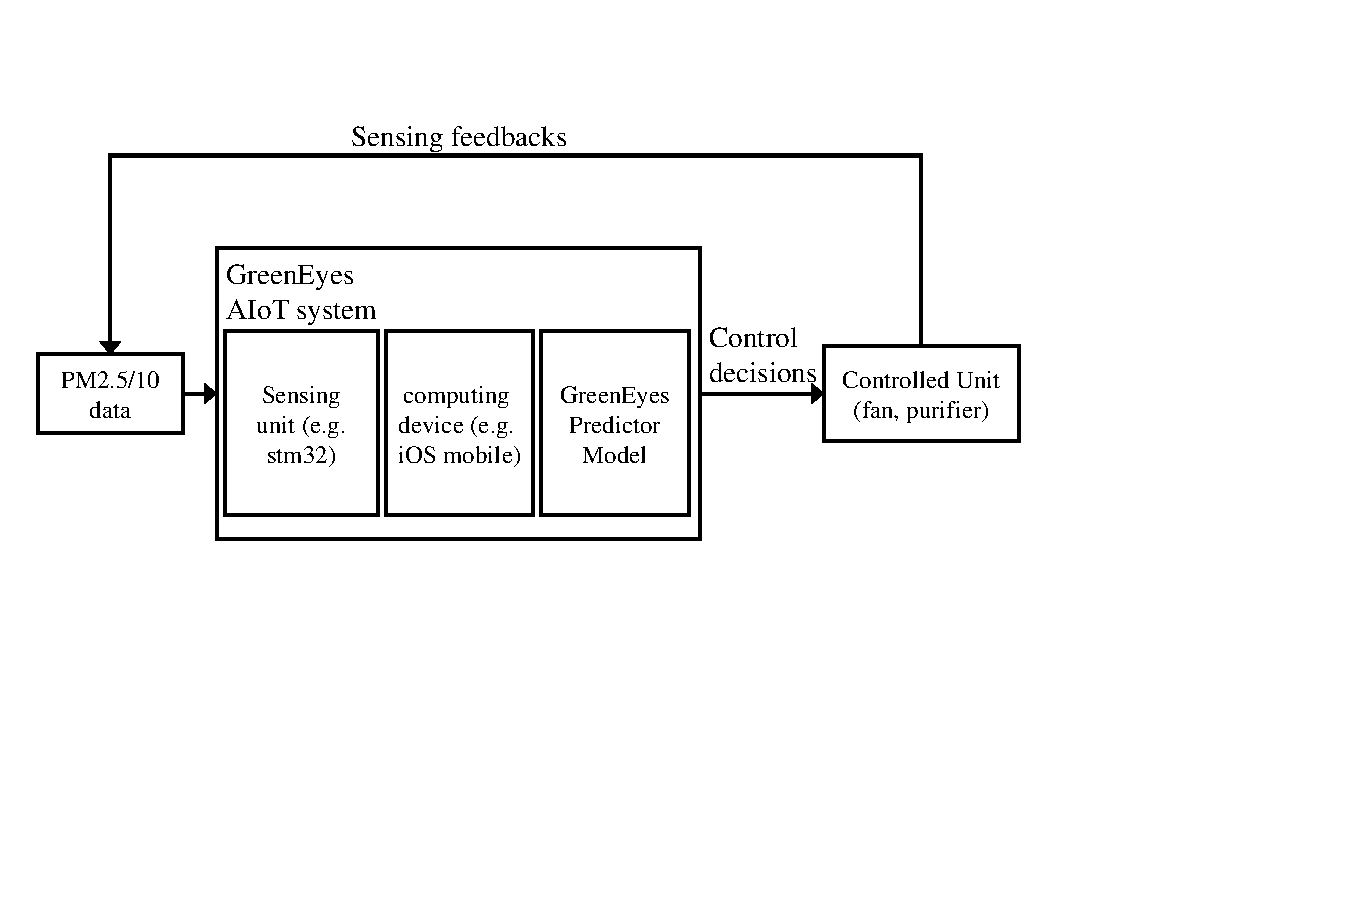
\includegraphics[width=\linewidth]{fig/aiot/greeneyes_aiot.pdf}
    \end{center}
    \caption{GreenEyes: AIoT deployment.}
    \label{fig:greeneyes_aiot}
\end{figure}

In this work, we firstly investigate the problem of preprocessing noisy PM2.5 sequence data and creating an appropriate supervising target sequence. We implement the GreenEyes model to predict the future air quality and evaluate it on each channel of PM2.5 data. Besides, we train our model with all channels' data together. Other works either use different kinds of data \cite{han2020joint}, or use sensors of the same model but place them at different places \cite{ray2016internet}. The former methodology is Multi-sensor Fusion \cite{wang2019multi}, it is widely used in the intelligent and autonomous systems \cite{luo1989multisensor, hall1997introduction, wang2012towards, cai2020probabilistic}. However, our approach of experiment proves that multi-sensors (of the same model, at the same place) will make the model perform better in predicting target data.

The main characteristics of this paper are summarized as follows:
\begin{itemize}
\item We treat WaveNet's residual layers as a feature block. This idea comes from the basic structures such as convolution-activation-pooling in computer vision. Such a design can increase reception filed and learn better representations.
%We believe that some modules can be generalized and used widely.
\item We innovatively stack several WaveNet blocks to build the model's main body. As the basic mechanism of deep learning networks is to build models brick by brick, the same module with different parameters is usually used in the same model. We borrow this idea and make it possible to parameterize our model. The model's optimal hyperparameters such as depth and filters can also be fine-tuned easily.
\item We put Attention \cite{bahdanau2014neural} and LSTM \cite{hochreiter1997long} at the endpoint as output layers. Ablation experiments demonstrate its necessity because this module can capture the hidden interations between features of different sequences (channels).
\end{itemize}

% The left part of this article will be organized by data modeling and model design, then experiment and conclusion.

\section{Datasets}\label{sec:data_modeling}

%The goal of our experimental evaluation is to guide the GreenEyes system to analyze the current status of ambient air quality and learn to make proper predictions. If possible, smart control actions such as  turning on\/off the air purrifier's fan could also be achieved. However, data processing in this section shows that 
AQI (\textbf{A}ir \textbf{Q}uality \textbf{I}ndex) is widely used for measuring the current pollution status of the air. IAQIs (\textbf{I}ndividual \textbf{A}ir \textbf{Q}uality \textbf{I}ndex) are calculated according to pollutants such as ozone, nitrogen dioxide, sulphur dioxide, and others, before final AQI is concluded. In our work, the IAQI of $PM_{2.5}$ is considered.

IAQI level data calculated from raw air quality data of sensors cannot be used directly because of high-frequency noise. As Figure \ref{fig:pm25_0_origin_and_labeled_level} presents, in some intervals of the time axis, the IAQI level fluctuates very fast. This is because the air quality data is exactly fluctuating around the threshold line. In real AIoT applications, we don't need this fluctuation. Image the following module is a fan switch that takes the model's output to determine and we want this output to be relatively stable. In order to clean the data fluctuation while keeping the trend features, we innovatively brought out a method of human manually labeling. It creates an appropriated target label function that the model can learn. Also, based on the labeling tricks, the problem that the predictions on the IAQI level will fluctuate near the thresholds is much reduced.

\subsection{Data Collection}

We placed our 4 sensors in an office room located inside the Academic Building of the HKUST. The room is inside the academic building and has no windows, it provides a stable experimental environment for temperature and humidity. The sampling rate of the sensor is 1 Hz. We simultaneously collected around 220k data points for each sensor in a continuous period starting from 20:28 on 25th November 2019. This period is about 2 days and a half or 61 hours.

\subsection{IAQI Calculation}

The final AQI depends on each pollutant's IAQI, which is calculated by Equation \ref{eq:IAQI_p}

\begin{equation}
    \label{eq:IAQI_p}
    IAQI_p = \frac{C_p-BP_{Lo}}{BP_{Hi}-BP_{Lo}}(IAQI_{Hi}-IAQI_{Lo})+IAQI_{Lo},
\end{equation}

and finally, AQI is calculated by Equation \ref{eq:AQI}
\begin{equation}
    \label{eq:AQI}
    AQI = \text{max}\{IAQI_{1}, IAQI_{2}, IAQI_{3}, ..., IAQI_{n}\}.
\end{equation}

In this paper, we only concern and discuss on the IAQI regarding $PM_{2.5}$.

% When it finally comes to AQI, for both China and USA standards, the maximum of these individual IAQI values\ref{formula:AQI} will be the AQI

% \begin{equation}
%     \label{formula:AQI}
%     AQI = \max\{IAQI_1,IAQI_2,IAQI_3,...,IAQI_n\}
% \end{equation}

Above equations about IAQI and AQI are universal for multi kinds of air pollution standards. Different thresholds are used when mapping air pollutants data into IAQI in different standards. Table \ref{table:IAQI_thresholds} lists $PM_{2.5}$ and $PM_{10}$ IAQI thresholds in China's and USA's standards respectively. In this paper, we use the \textbf{USA standard}. 

\begin{table}[!htbp]
    \centering
    \caption{Concentration thresholds of IAQI w.r.t. pollutant categories, USA}
    \label{table:IAQI_thresholds}
    \begin{tabular}{l|l|l|l|l}
        \hline
        \hline
        \  & USA & USA & China & China \\ \hline
        IAQI & \makecell[c]{$PM_{2.5}$ \\ ($\mu g/m^3$)} & \makecell[c]{$PM_{10}$ \\ ($\mu g/m^3$)} & \makecell[c]{$PM_{2.5}$ \\ ($\mu g/m^3$)} & \makecell[c]{$PM_{10}$ \\ ($\mu g/m^3$)} \\ \hline
        0    & 0     & 0   & 0   & 0   \\ \hline
        50   & 12.1  & 55  & 35  & 50  \\ \hline
        100  & 35.5  & 155 & 75  & 150 \\ \hline
        150  & 55.5  & 255 & 115 & 250 \\ \hline
        200  & 150.5 & 355 & 150 & 350 \\ \hline
        300  & 250.5 & 425 & 250 & 420 \\ \hline
        400  & N/A   & N/A & 350 & 500 \\ \hline
        500  & 500.4 & 604 & 500 & 600 \\ \hline
        \hline
    \end{tabular}
\end{table}

Figure \ref{fig:pm25_all_iaqi_with_thresholds} shows the IAQI curves corresponding to $PM_{2.5}$, with thresholds lines.

\begin{figure*}[!htbp]
    \begin{center}
        
\includegraphics[width=0.8\linewidth]{fig/data/iaqi/pm25_all_iaqi_with_thresholds.png}
    \end{center}
    \caption{All $PM_{2.5}$ data with IAQI thresholds.}
    \label{fig:pm25_all_iaqi_with_thresholds}
\end{figure*}

\subsection{Data Polynomialization}

The task of our model is to predict the IAQI level when inputting a segment of air pollutant concentration data. However, the origin IAQI level lines cannot be directly used because 1. in deep learning, a step function is very hard to learn especially on the rising and falling edges; 2. in some areas the IAQI level fluctuates extremely frequently, which makes the learning even harder, as shown in Figure \ref{fig:pm25_0_origin_and_labeled_level}.

% \begin{enumerate}
%     \item Direct learning on the origin IAQI level is equivalant to learning the IAQI and its level formula. This is not necessary and not novel.
%     \item The IAQI level lines are actually consisted of series of level step step-downs/ups. In deep learning, a step function is every hard to learn. \item Moreover, as Figure \ref{fig:pm25_0_origin_and_labeled_level} shows, in some area the IAQI level fluctuates extreme frequently, which makes the learning even harder. These frequent fluctuations are actually due to the air pollutant's concentration value floats near its thresholds. This kind of floating causes \textbf{hesitation} phenomena for our model to predict.
% \end{enumerate}

We're inspired by B. Rouet-Leduc's work \cite{rouet2017machine} on earthquake predicting, where the earthquake events are represented as failures. The target function is designed as a series of descending ramps. Mathematically, these descending ramps form a polygonal function and count down the time to next earthquake. The problem is turned into fitting the time counting down curve with the acoustic data input.

A polygonal function, also named piece-wise linear function $f(x)$, is a continuous function mathematically defined on an interval $[a, b]\in \mathbb R$ such that $[a, b]$ can be divided into a set of intervals on each of which the function is a linear function, that is, there exists a subdivision 
\begin{equation}
    a=x_0 < x_1 < ... < x_n=b
\end{equation}
such that $f(x)$ is linear on each interval $[x_{n-1}, x_n]$.

Polygonal functions can be used to generate approximations to known curves, planes, etc. Also, for unknown data, polygonal functions can also be learned by some algorithms such as decision tree, to fit the data. In our work of predicting, polygonal functions help us to eliminate the \textbf{hesitation} area, and build the target data.

\subsection{Data Polygonalization: Human Labeling based on Decisions}

We firstly label by hand the level step down\/up points, and map them into rising\/falling lines. This method transfer discrete decision points into continuous target data series which have the same dimension as the time indices and corresponding $PM_{2.5}$ data. This kind of method make us get the polygonal target data as B. Rouet-Leduc, et al. \cite{rouet2017machine} did. Figure \ref{fig:pm25_0_origin_and_labeled_level} shows our labeling results.

\begin{figure*}[!htbp]
    \begin{center}
        
\includegraphics[width=0.8\linewidth]{fig/data/labeled_iaqi_level/origin_and_labeled/pm25_0.png}
        \caption{Sensor 0's $PM_{2.5}$ origin and labeled IAQI level.}
        \label{fig:pm25_0_origin_and_labeled_level}
    \end{center}
\end{figure*}

% \begin{equation}
%     Level_t = (Level_{end}-Level_{begin}) / t-t_{begin}
% \end{equation}

Finally, the labeled target data is turned into a polygonal function. Dash lines in Figure \ref{fig:pm25_0_labeled_level} shows the results. These triangular lines will be label data for our supervised learning fitting problem.

\begin{figure*}[!htbp]
    \centering
    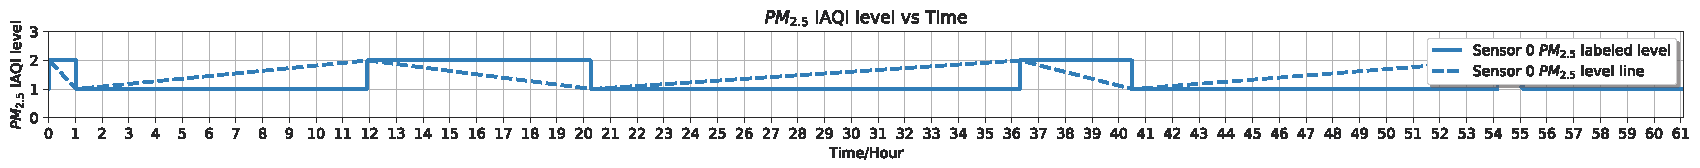
\includegraphics[width=0.8\linewidth]{fig/data/labeled_iaqi_level/pm25_0_labeled_iaqi_level.png}
    \caption{Sensor 0's labeled $PM_{2.5}$ IAQI level and its polygonal line.}
    \label{fig:pm25_0_labeled_level}
\end{figure*}

The level polygonal lines w.r.t. their manually labeled level curves can be written as equations with form below
\begin{equation}
    \label{formula:polygonal}
    L_i(t)=k_i*t+b_i,\ where\ t\in[t_i,t_{i+1}],
\end{equation}
where $k_i$ is the slope of the curve, $t_i$ and $t_{i+1}$ are start and end time point for every interval of the polygonal line. When $k_i>0$, the trend of the IAQI level is raising, and vice versa. The absolute value of $k_i$ is the approximate and potential changing speed of IAQI level. Thus, every polygonal line can be divided into several segments within time interval $t_i$ to $t_{i+1}$, and every segment estimates the 1-order approximate trend w.r.t. original IAQI level within corresponding time interval. For the i-th segment, $k_i$ is
\begin{equation}
    k_i = \frac{l_{i+1}-l_i}{t_{i+1}-t_i}.
\end{equation}
where $l_{i+1}$ and $l_i$ are the original IAQI levels at end and start time $t_{i+1}$ and $t_i$.

Our experiments will take these polygonalized IAQI level lines as the supervising data. The fitting problem can be described as: given a IAQI sequence of \textit{windows size}, predict the IAQI level of the next time frame after this time window.


\section{Methodology}\label{sec:model_design}

\begin{figure*}[!htbp]
  \centering
  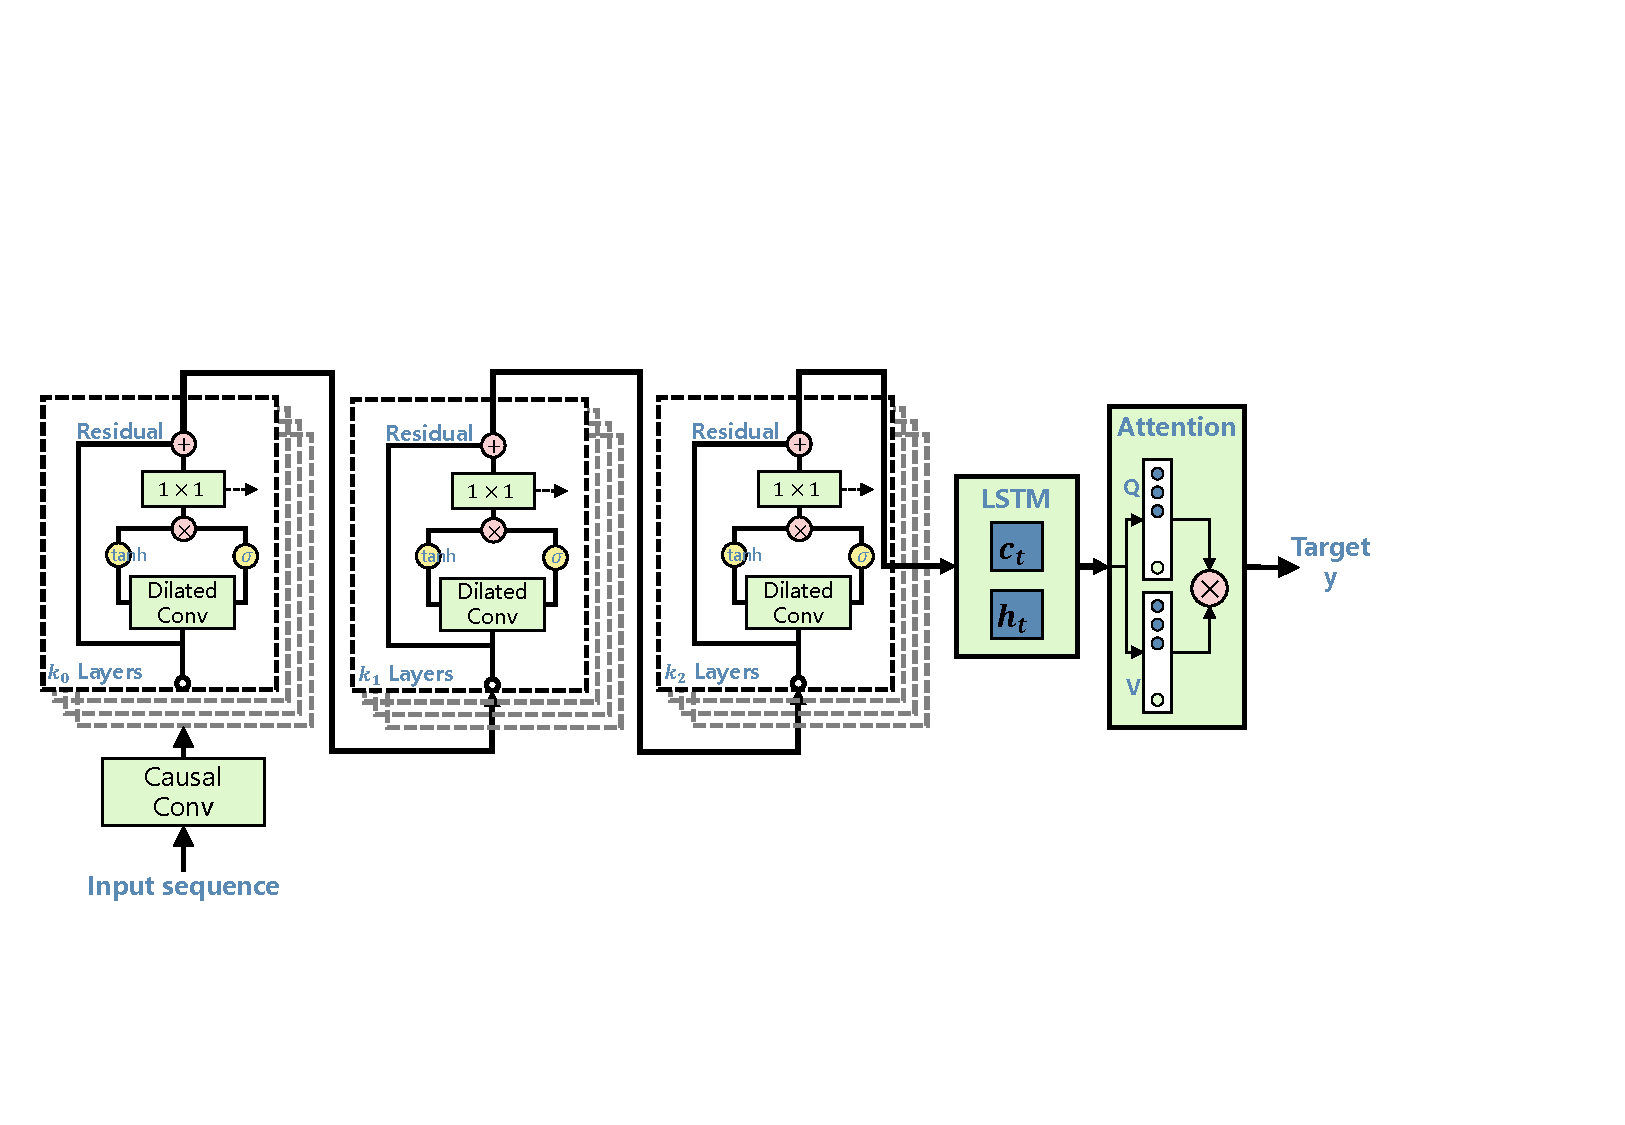
\includegraphics[width=0.8\linewidth]{fig/model/WaveNet_LSTM_ver0.1.pdf}
  \caption{GreenEyes sequence to point fitting model.}
  \label{fig:greeneyes_model}
\end{figure*}

% audio applications such as speech synthesis  have been developed. 
% They introduce a new generative model operating directly on the raw audio waveform. 
Recently, a series of neural networks related to the auto-regression model has been proposed and applied in regarding problems. DeepMind's WaveNet \cite{oord2016wavenet} is one of the famous and foundation work in between those \cite{shen2018natural}, \cite{wang2017tacotron} tackle with sequence representation and generating. For WaveNet's application scenario, the joint probability of the target sequence $\textbf{x}=\{x_1,x_2,...,x_T\}$ is factorized as a product of conditional probabilities as the below Equation \ref{eq:auto-regression-model}. Given an input $\bar{\textbf{x}}=\{x_1,x_2,...,x_{T-1}\}$ and with this conditional probabilities, we can obtain the distribution of the value $x_T$, and make generation samples.

\begin{equation}
    p(\textbf{x})=\prod_{t=1}^Tp\{x_t|x_1,x_2,...,x_{t-1}\}
    \label{eq:auto-regression-model}
\end{equation}

Auto-regression models can not only be used in data generation, but also in time series prediction. In our work, every sample $x_t$ and $y_t$ at any time step $t$ is conditioned on the samples at all previous timestamps, making it a multivariate auto-regression task. To limit the input length,  we only consider the conditional probabilities between $x_t$ and a sequence $x_{t-1-window\_size:t-1}$ with length $window\_size$. Different with other multivariate auto-regression tasks where sequences on all the temporal axis are modeled, we haven't used the sequence $y_{t-1-window\_size:t-1}$ to predict $y$, instead, we predict $y$ only with $x_{t-1-window\_size:t-1}$.

% TODO
Different from B. Rouet-Leduc's work\cite{rouet2017machine}, in which random forest is used to predict seismic precursors, we use WaveNet as our GreenEyes model's main part. Air pollution data has the same structure as audio data. It is pretty suitable to utilize WaveNet as air pollution data can be modeled in the same way. Also, WaveNet's dilated causal convolutions and residual and skip connections are suitable for air pollution data.

We used the original WaveNet's core part as a WaveNet Block as we believe this block\-style configuration is more modularized, for we could change these blocks' hyper parameters more easily. Each WaveNet Block, as the same with WaveNet, contains several dilated convolution layers, called WaveNet Layer. Different dilation rates are also set on them, following DeepMind's original work. 

The designing of neural networks for deep learning has always followed principles such as modularization, and expandability. Well-known networks, such as VGG \cite{simonyan2014very} and ResNet \cite{he2016deep}, all have these features. VGG has two model types VGG16, and VGG19, with different model depth. And ResNet has models ResNet-18, ResNet-34, ResNet-50, etc. The cutting-edge model, Transformer \cite{vaswani2017attention}, also obeys these designs which makes it possible to build multi variant models for various sizes and application scenarios. Our model is designed for parameterization, too. Following our constructions, finally we set 8 WaveNet layers for the first block; and 5 layers for the second, 3 layers for the third. All blocks share the same kernel size of 3, and filters of 16. This set of hyper parameters are chosen by empiric and the computational capability of a 1080 Ti GPU. There might be more optimal parameters to search in future works.

As for the Attention layer, we set up two kinds of Attention mechanism - Dot-product attention layer, a.k.a. Luong-style attention \cite{luong2015effective}, as Equation \ref{eq:dot-product-attention} shows. We use the input for all value vector, key vector, and query input. Another mechanism is made by ourselves, called Temporal Attention. 

\begin{gather}
    \text{scores}=QK^T \\
    \text{Attention}(Q, K, V ) = \text{softmax}(QK^T)V
    \label{eq:dot-product-attention}
\end{gather}

In our Attention layer, we still use the Luong's multiplicative style attention \ref{eq:Luong-multiplicative-style} to gain score, but we simply it with a FC network. Moreover, we don't use softmax function to compute the attention weight. Rather, we use the function as Equation \ref{eq:temporal-attention} shows.

\begin{equation}
    \text{scores}(\bar {\textbf{\textit h}}_t^T,\bar {\textbf{\textit h}}_s)=\bar {\textbf{\textit h}}_t^T\textbf{\textit W}\bar {\textbf{\textit h}}_s 
    \label{eq:Luong-multiplicative-style}
\end{equation}

\begin{gather}
    \text{scores}=\textbf{\textit W}\textbf{\textit V}+\textbf{\textit b} \\
    \text{Attention}(V) = \text{exp}(\text{tanh}(\text{scores}))V
    \label{eq:temporal-attention}
\end{gather}

The reason that we replace the softmax with a tanh function followed by an exponential function, is to better adapt our model to the temporal data set. Our data set have many temporal and periodic features to learn. Tanh function is very common in sequential models, and it is also a component in every WaveNet layer.

\section{Experiments}

\subsection{Experimental Settings}

% 描述实验的组别,个数
As we sampled $PM_{2.5}$ measurements from 4 sensors, Sensor 0 to Sensor 3, so we have a 4-channels $PM_{2.5}$ IAQI data set. Each channel's data can be taken as an individual data set. The stride is set as $\{10, 5, 2\}$, respectively. Besides, we fuse data from all channels to create a new data set named $PM2.5_{All}$.

%And there are 3 different stride values, so finally we have 12 experiments to perform for each configuration of the model. Besides, we have a group of augmentation experiments in which all 4 sensors' data are fed to the model, yielding another 3 experiments with different stride parameters. The augmented data with all the channels can also be treated as a new data set, as called $PM2.5_{All}$.
% LR 配置
Adam\cite{kingma2017adam} optimizer with an initial learning rate 0.0001 is applied in the experiments, which is multiplied by 0.1 after 20 epochs, where the total training epoch is 100.
% Loss 配置
We use mean squared error (MSE) and mean absolute error (MAE) as the evaluation metrics.

% They are defined by equations below
% \begin{equation}
%     MSE(p, y)=E((p_i-y_i)^2)
% \end{equation}
% \begin{equation}
%     MAE(p, y)=E(|p_i-y_i|)
% \end{equation}
% where $p$ is the prediction sequence and $y$ is the polygonalized $PM_{2.5}$ IAQI sequence.
% 4 metrics: , mean squared error (MSE), mean absolute percentage error (MAPE), mean squared logarithmic error (MSLE).

\subsection{Training and Validation} % 15 experiments

\subsubsection{Why did We Redesign the Attention Layer?}

At first, we utilized the dot-product attention layer provided by TensorFlow official. Table \ref{table:best_metrics_official_training} lists all the experiments' final best metrics during training.

\begin{table}[!htbp]
    \centering
    \begin{tabular}{c|c|c|c}
        \hline\hline
        Data & Stride & \makecell[c]{Minimum \\ train MSE} & \makecell[c]{Minimum \\ validation MSE} \\\hline
        \multirow{3}{*}{\text{$PM_{2.5}$(0)}} & 10 & 0.0969 & 0.1221 \\ \cline{2-4} 
                                        & 5 & 0.0071 & 0.0221 \\ \cline{2-4} 
                                        & 2 & 0.0049 & 0.0148 \\ \hline
        \multirow{3}{*}{\text{$PM_{2.5}$(1)}} & 10 & 0.0148 & 0.0226 \\ \cline{2-4} 
                                        & 5 & 0.0062 & 0.0137 \\ \cline{2-4} 
                                        & 2 & 0.0006 & 0.0039 \\ \hline
        \multirow{3}{*}{\text{$PM_{2.5}$(2)}} & 10 & 0.0087 & 0.0137 \\ \cline{2-4} 
                                        & 5 & 0.0080 & 0.0153 \\ \cline{2-4} 
                                        & 2 & 0.0027 & 0.0154 \\ \hline
        \multirow{3}{*}{\text{$PM_{2.5}$(3)}} & 10 & 0.0123 & 0.0209 \\ \cline{2-4} 
                                        & 5 & 0.0058 & 0.0110 \\ \cline{2-4} 
                                        & 2 & 0.0023 & 0.0037 \\ \hline
        \multirow{3}{*}{\text{$PM_{2.5}$(All)}} & 10 & 0.0182 & 0.0266  \\ \cline{2-4} 
                                        & 5 & 0.0039 & 0.0053 \\ \cline{2-4} 
                                        & 2 & 0.0010 & 0.0005 \\
        \hline
        \hline
    \end{tabular}
    % \caption{\textcolor{red}{Best metrics during training when applying official Attention.}}
    \caption{Best metrics during training when applying official Attention.}
    \label{table:best_metrics_official_training}
\end{table}

After we train the model with Temporal Attention, we discovery that the results on official Attention show limitations and defects. As Table \ref{table:best_metrics_myattention_training} shows, in most experiments, Temporal Attention outperforms official Attention. When we plot the validation curve, some principles can be figured out, specifically, Figure \ref{fig:val_mse_official} illustrates the validation MSE's curves with $stride=10$, and Figure \ref{fig:val_mse_myattention} illustrates the validation MSE's curves when applying Temporal Attention. We can conclude that when applying official Attention, the model cannot converge consistently with different data sets. Figure \ref{fig:val_mse_official} shows that model fails to converge when it learns on \text{$PM_{2.5}$(0)}. Meanwhile, applying Temporal Attention, the model can obtain a better MSE.
% Curves when stride is set 5 and 2 can be found in the appendix. 

% Validation curves, official Attention
\begin{figure}[!htbp]
    \centering
    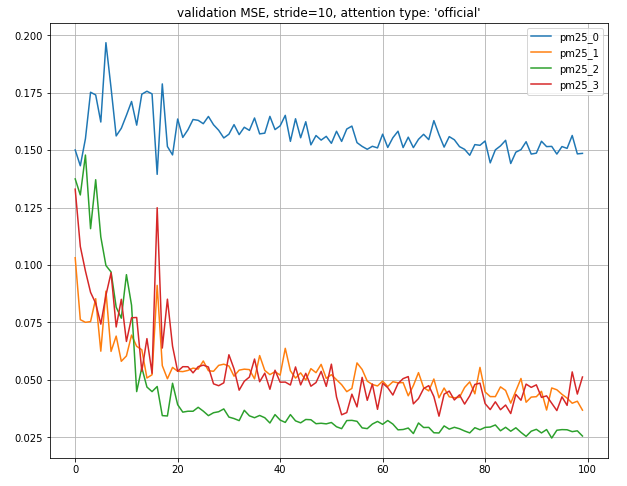
\includegraphics[width=0.8\linewidth]{fig/results/validation/val_mse_official.png}
    \caption{Validation MSE curves when applying official Attention ($stride=10$).}
    \label{fig:val_mse_official}
\end{figure}

% Validation curves, Temporal Attention
\begin{figure}[!htbp]
    \centering
    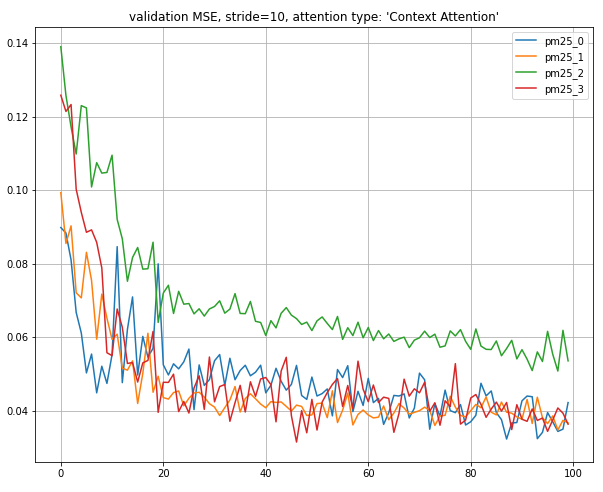
\includegraphics[width=0.8\linewidth]{fig/results/validation/val_mse_myattention.png}
    \caption{Validation MSE curves when applying Temporal Attention ($stride=10$).}
    \label{fig:val_mse_myattention}
\end{figure}

% \begin{figure}[!htbp]
%     \centering
%     \begin{subfigure}{0.3\linewidth}
%         \centering
%         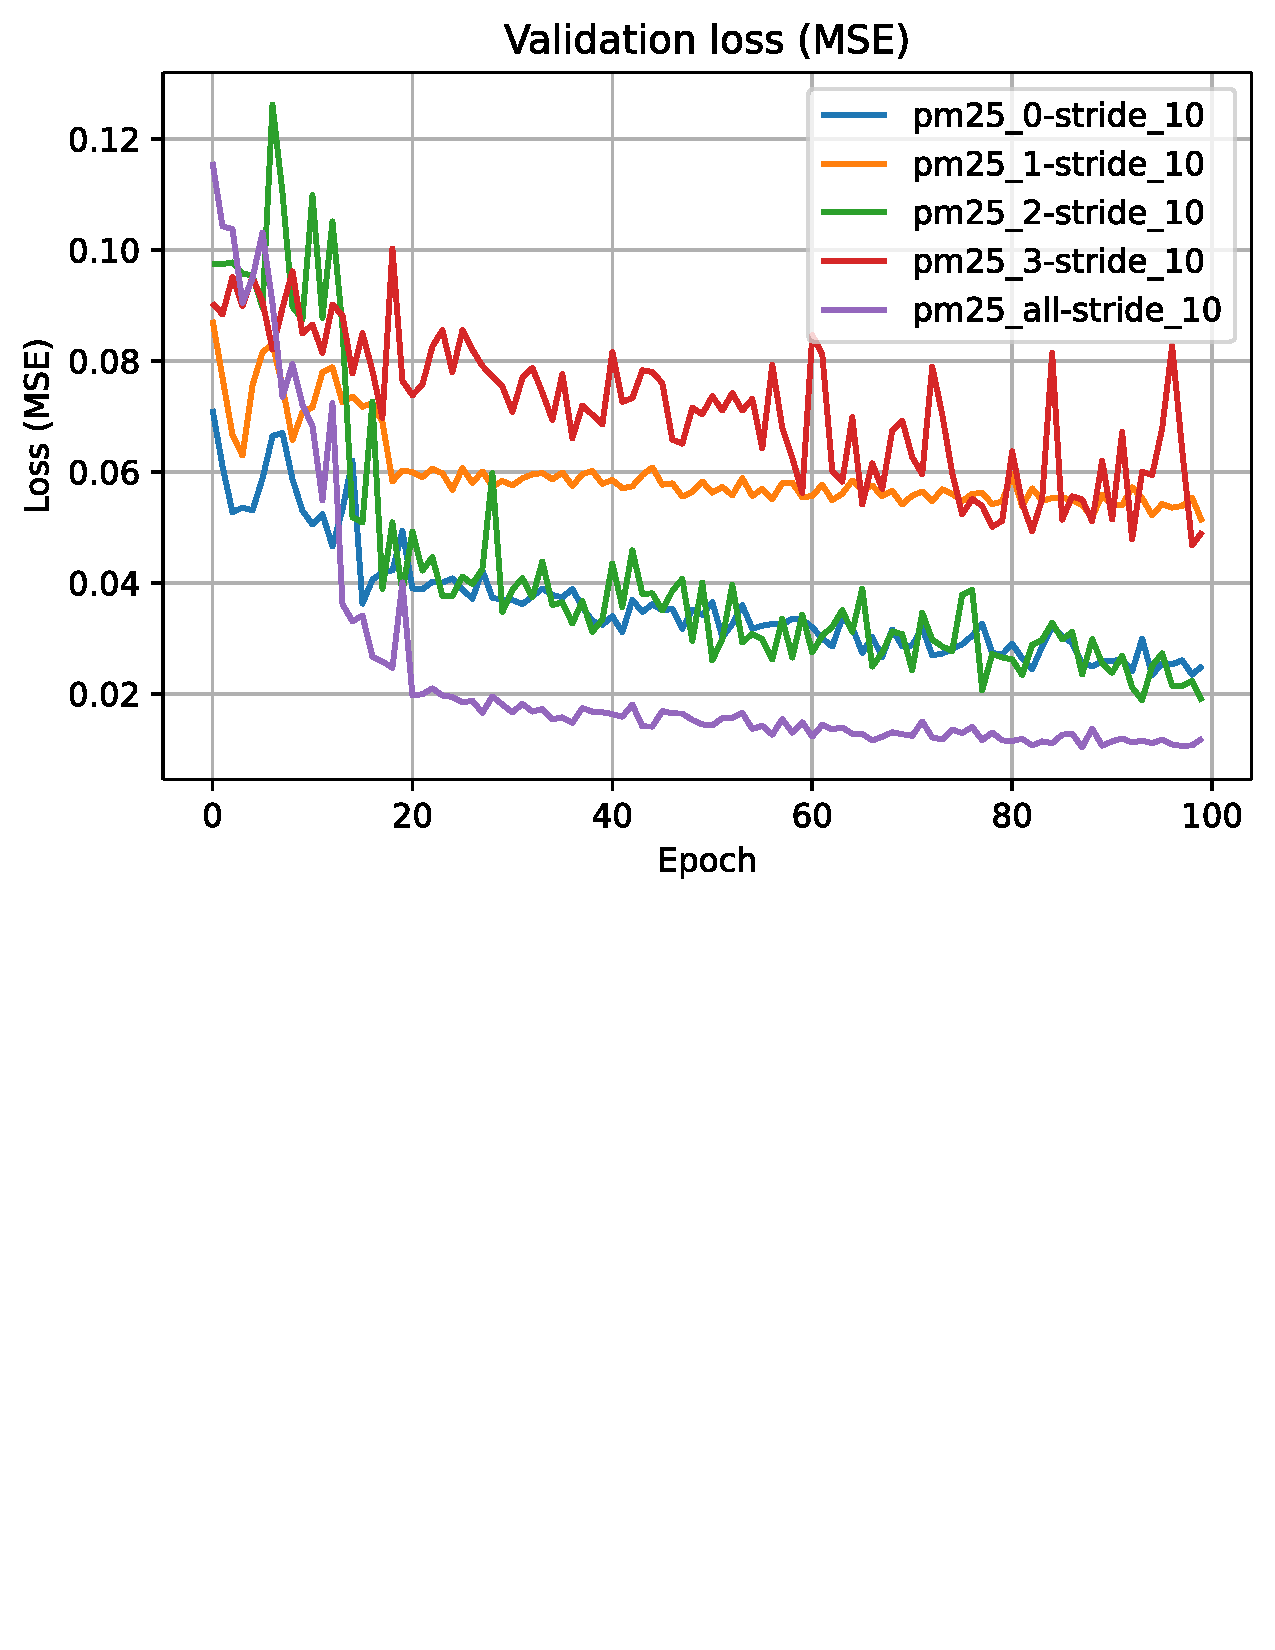
\includegraphics[width=\linewidth]{fig/results/val_curves_stride_10.pdf}
%         \caption{stride=10.}
%         \label{fig:val_stride_10}
%     \end{subfigure}
%     \hfill
%     \begin{subfigure}{0.3\linewidth}
%         \centering
%         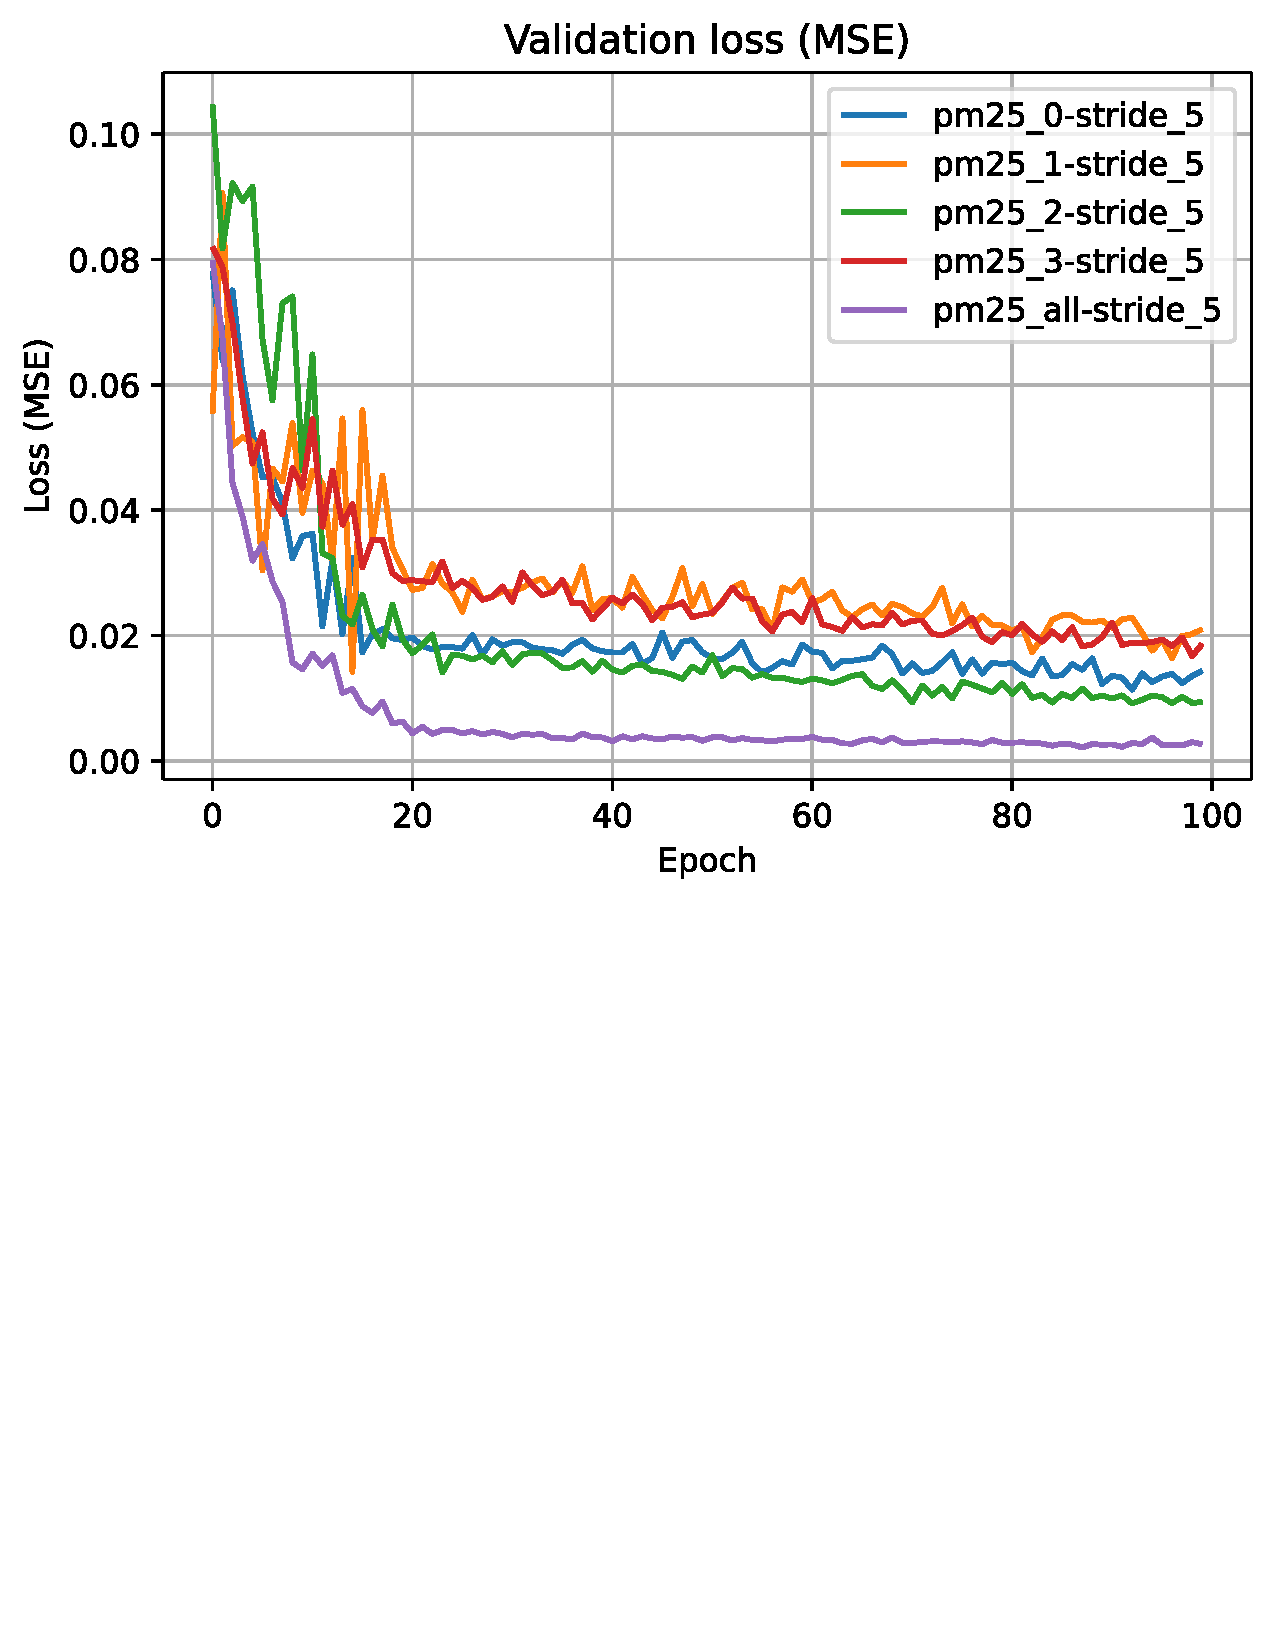
\includegraphics[width=\linewidth]{fig/results/val_curves_stride_5.pdf}
%         \caption{stride=5.}
%         \label{fig:val_stride_5}
%     \end{subfigure}
%     % \hfill
%     \begin{subfigure}{0.3\linewidth}
%         \centering
%         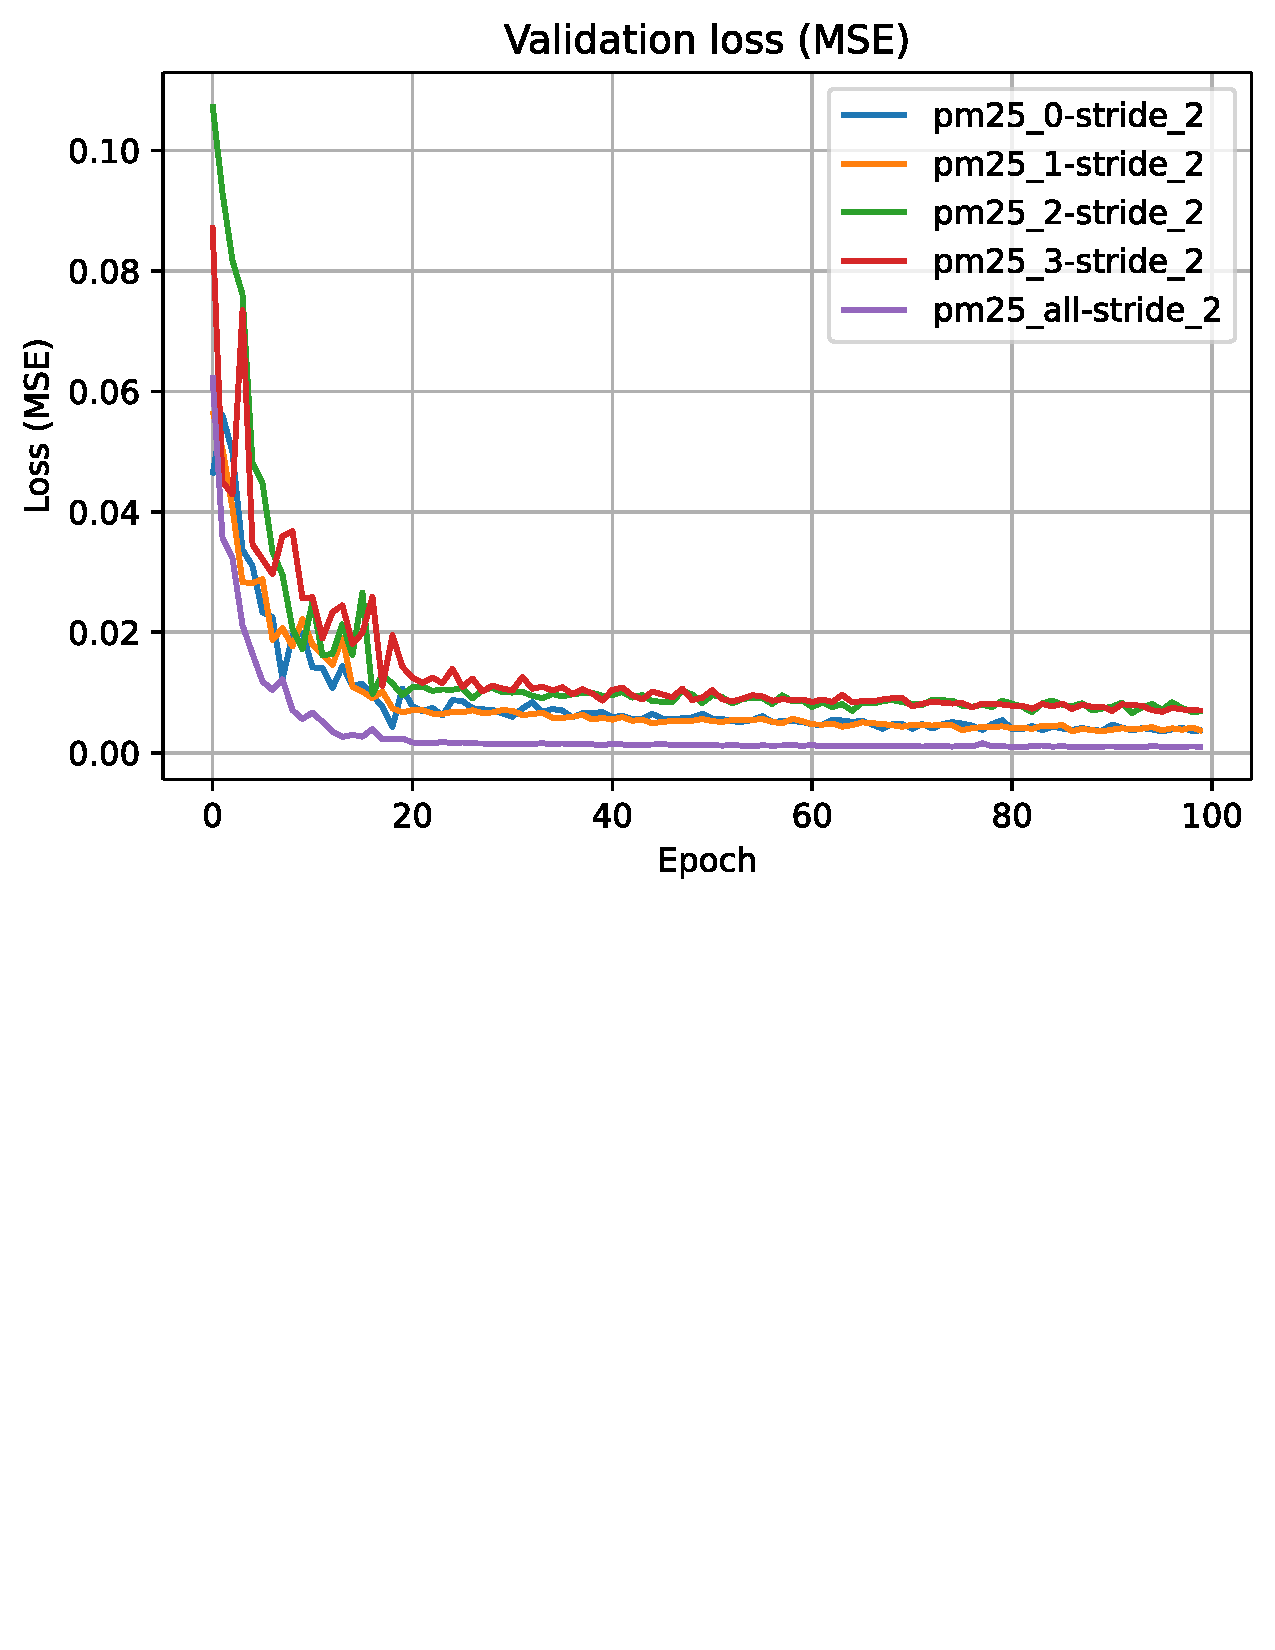
\includegraphics[width=\linewidth]{fig/results/val_curves_stride_2.pdf}
%         \caption{stride=2.}
%         \label{fig:val_stride_2}
%     \end{subfigure}
% \caption{Validation MSE curves.}
% \label{fig:val_mse}
% \end{figure}

\subsubsection{Best Metrics during Training}

% As we used MSE as loss, i.e. the supervising metric, we extracted minimum train MSE and minimum validation MSE from all the training epochs. These best metrics reflect the model's fitting results. They are all rounded to 4 decimals. 

% We also record other metrics such as MAE during training.

% After changing official Attention to Temporal Attention, we obtained each experiment's final best metrics during training as Table \ref{table:best_metrics_myattention_training} lists.
Table \ref{table:best_metrics_myattention_training} shows the experimental best metrics during training with the proposed Temporal Attention. It is obvious that in most cases, our Attention outperforms the official Attention. We also define a coefficient $ratio=\frac{min(train\ MSE)}{min(validation\ MSE)}$ to simply measure the generalization capability of the model.
%during certain an experiment.

\begin{table}[!htbp]
    \centering
    \begin{tabular}{c|c|c|c|c}
        \hline\hline
        Data & Stride & \makecell[c]{Minimum \\ train MSE} & \makecell[c]{Minimum \\ validation MSE} & ratio \\\hline
        \multirow{3}{*}{\text{$PM_{2.5}$(0)}} & 10 & 0.0223 & 0.0234 & 0.96 \\ \cline{2-5} 
                                        & 5 & 0.0034 & 0.0114 & 0.30 \\ \cline{2-5} 
                                        & 2 & \textbf{\textit{0.0006}} & \textbf{\textit{0.0035}} & 0.16 \\ \hline
        \multirow{3}{*}{\text{$PM_{2.5}$(1)}} & 10 & 0.0486 & 0.0510 & 0.95 \\ \cline{2-5} 
                                        & 5 & 0.0058 & 0.0142 & 0.41 \\ \cline{2-5} 
                                        & 2 & \textbf{\textit{0.0006}} & \textbf{\textit{0.0036}} & 0.17 \\ \hline
        \multirow{3}{*}{\text{$PM_{2.5}$(2)}} & 10 & 0.0171 & 0.0187 & 0.92 \\ \cline{2-5} 
                                        & 5 & 0.0024 & 0.0092 & 0.27 \\ \cline{2-5} 
                                        & 2 & \textbf{\textit{0.0012}} & \textbf{\textit{0.0066}} & 0.19 \\ \hline
        \multirow{3}{*}{\text{$PM_{2.5}$(3)}} & 10 & 0.0509 & 0.0468 & 1.09 \\ \cline{2-5} 
                                        & 5 & 0.0074 & 0.0167 & 0.44 \\ \cline{2-5} 
                                        & 2 & \textbf{\textit{0.0010}} & \textbf{\textit{0.0068}} & 0.15 \\ \hline
        \multirow{3}{*}{\text{$PM_{2.5}$(All)}} & 10 & 0.0068 & 0.0103 & 0.66 \\ \cline{2-5} 
                                        & 5 & 0.0014 & 0.0022 & 0.67 \\ \cline{2-5} 
                                        & 2 & \textbf{0.0007} & \textbf{0.0009} & 0.77 \\
        \hline
        \hline
    \end{tabular}
    % \caption{\textcolor{red}{Best metrics during training when applying Temporal Attention.}}
    \caption{Best metrics during training when applying Temporal Attention.}
    \label{table:best_metrics_myattention_training}
\end{table}

\subsection{Model Evaluation}

% Evaluation curves
\begin{figure*}[!htbp]
    \centering
    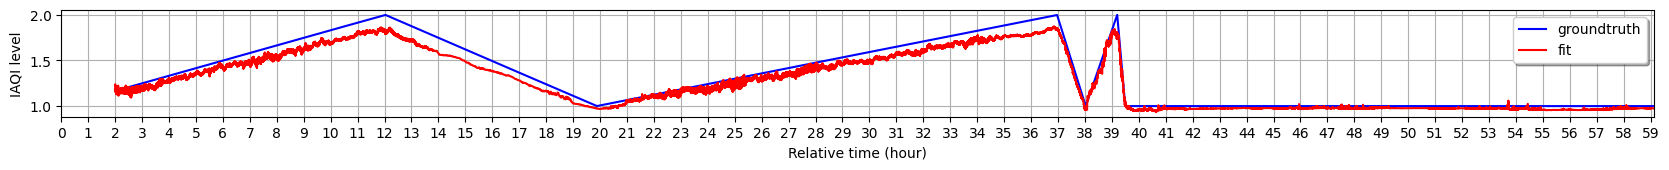
\includegraphics[width=\linewidth]{fig/results/evaluation/model_eval_pm25_3_stride_5.png}
    \caption{Evaluation of the GreenEyes model (\text{$PM_{2.5} (3)$}, stride=5).}
    \label{fig:model_eval_pm25_3_stride_5}
\end{figure*}

\begin{figure*}[!htbp]
    \centering
    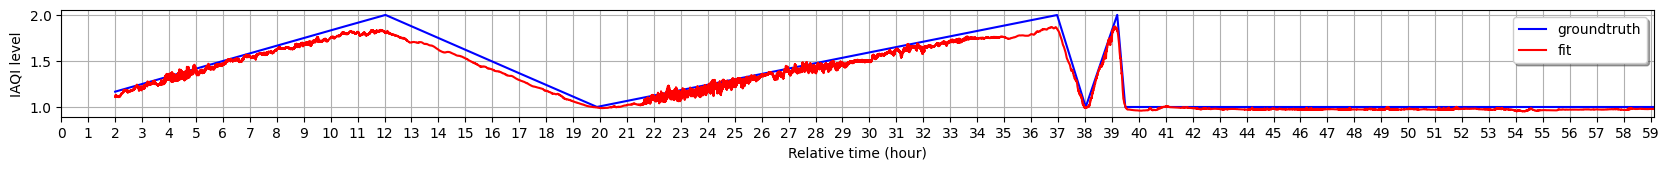
\includegraphics[width=\linewidth]{fig/results/evaluation/model_eval_pm25_3_stride_2.png}
    \caption{Evaluation of the GreenEyes model (\text{$PM_{2.5} (3)$}, stride=10).}
    \label{fig:model_eval_pm25_3_stride_2}
\end{figure*}

Figure \ref{fig:model_eval_pm25_3_stride_5} shows that our model fits the labeled IAQI level lines well, except that its predictions differ from the ground truth a little on some parts of the lines, especially on the turning corners. Figure \ref{fig:model_eval_pm25_3_stride_2} illustrates the same evaluation performance, which presents that the model may not need much data to learn as to set stride to 2.
To quantify the testing results of our model with different parameters, we test it on the whole $PM_{2.5}$ sequence by setting stride as 1. Table \ref{table:test_mse_mae} lists the statistics of our tests.

% We performed the tests using two metrics, mean square error (MSE) and mean absolute error (MAE).
% And we test all models trained under different stride parameter and on every channel of $PM_{2.5}$ data. 
% Future: 更换为新的实验数据

\begin{table}[!htbp]
    \centering
    \begin{tabular}{c|c|c|c}
        \hline\hline
        Data & Stride & MSE & MAE \\\hline
        \multirow{3}{*}{\text{$PM_{2.5}$(0)}} & 10 & 0.0266 & 0.13 \\ \cline{2-4} 
                                        & 5 & 0.0144 & 0.11 \\ \cline{2-4} 
                                        & 2 & \textbf{\textit{0.0037}} & \textbf{\textit{0.05}} \\ \hline
        \multirow{3}{*}{\text{$PM_{2.5}$(1)}} & 10 & 0.0517 & 0.18 \\ \cline{2-4} 
                                        & 5 & 0.0113 & 0.10 \\ \cline{2-4} 
                                        & 2 & \textbf{\textit{0.0036}} & \textbf{\textit{0.05}} \\ \hline
        \multirow{3}{*}{\text{$PM_{2.5}$(2)}} & 10 & 0.0188 & 0.11 \\ \cline{2-4} 
                                        & 5 & 0.0092 & 0.09 \\ \cline{2-4} 
                                        & 2 & \textbf{\textit{0.0069}} & \textbf{\textit{0.07}} \\ \hline
        \multirow{3}{*}{\text{$PM_{2.5}$(3)}} & 10 & 0.0501 & 0.16 \\ \cline{2-4} 
                                        & 5 & 0.0108 & 0.09 \\ \cline{2-4} 
                                        & 2 & \textbf{\textit{0.0070}} & \textbf{\textit{0.07}} \\ \hline
        \multirow{3}{*}{\text{$PM_{2.5}$(All)}} & 10 & 0.0118 & 0.09 \\ \cline{2-4} 
                                        & 5 & 0.0026 & 0.04 \\ \cline{2-4} 
                                        & 2 & \textbf{0.0010} & \textbf{0.02} \\ \hline
        \hline
    \end{tabular}
    \caption{Test MSE and MAE under different stride parameter.}
    \label{table:test_mse_mae}
\end{table}

\subsection{Ablation Study}

In order to validate the effectiveness of the modules, we conduct an ablation study on our GreenEyes model. We remove the bidirectional LSTM module and the mutli-head attention module, respectively, and get two model variance, w/o Attention and w/o LSTM. We plot the model's (w/o LSTM) training and validation curves as Figure and Figure show respectively.

\begin{figure}[!htbp]
    \centering
    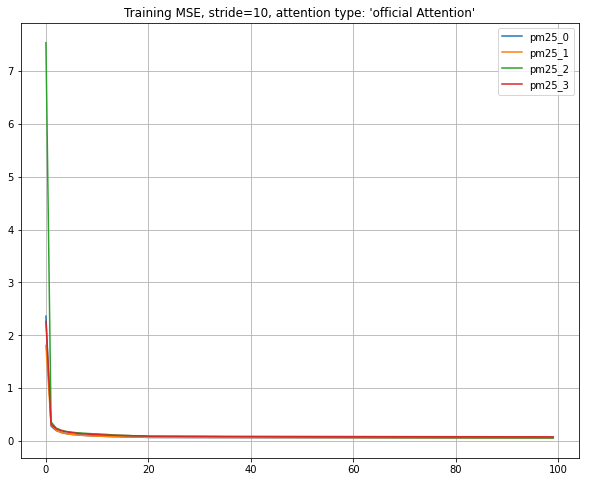
\includegraphics[width=0.6\linewidth]{fig/results/ablation/wo-LSTM-training.png}
    \caption{Model's (w/o LSTM) training plots (stride=10).}
    \label{fig:wo-LSTM-training}
\end{figure}

\begin{figure}[!htbp]
    \centering
    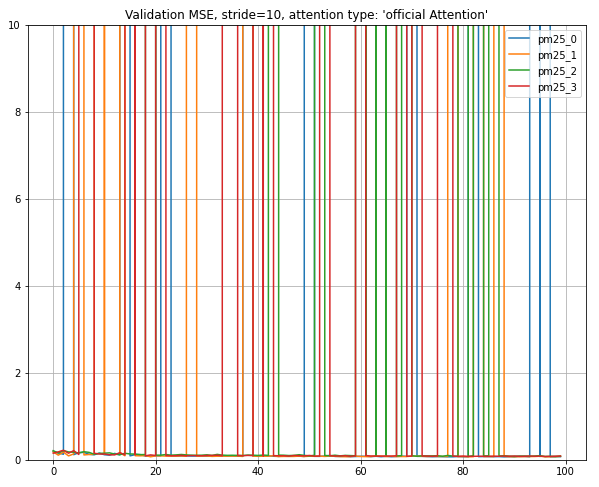
\includegraphics[width=0.6\linewidth]{fig/results/ablation/wo-LSTM-validation.png}
    \caption{Model's (w/o LSTM) validating plots (stride=10).}
    \label{fig:wo-LSTM-validation}
\end{figure}

It is easily concluded that, without the LSTM layer, the model runs into the overfit status. Although it still fits well on the train set, it is rambling on the validation set.

In order to validate the Attention layer's function, we re-run the GreenEyes model with Temporal Attention on \text{$PM_{2.5}$(0)} to \text{$PM_{2.5}$(3)}, and then cut off this Attention layer and run the model again on the same data sets. Table \ref{table:myattention_vs_no_attention} shows the test MSE and MAE results of both configuration. It turns out that the model w/o Attention can perform better or is equivalent to the model applied with the Attention layer. However, by plotting the training curves again, we found that the model with the Temporal Attention layer can obtain smaller loss during training. 

\begin{table}[!htbp]
    \centering
    \begin{tabular}{c|c|c|c|c|c}
    \hline\hline
     & & \multicolumn{2}{c}{Our Attention} & \multicolumn{2}{c}{w/o Attention} \\ \cline{3-6}
    \multirow{-2}{*}{Data} & \multirow{-2}{*}{Stride} & MSE & MAE & MSE & MAE \\ \hline
    \multirow{3}{*}{\text{$PM_{2.5}$(0)}} & 10 & 0.0267 & 0.1438 & \textbf{0.0173} & \textbf{0.1189} \\ \cline{2-6}
      & 5 & 0.0119 & 0.1011 & \textbf{0.0092} & \textbf{0.0795} \\ \cline{2-6}
      & 2 & \textbf{0.0055} & \textbf{0.0661} & 0.0078 & 0.0721 \\ \cline{2-6}
    \multirow{3}{*}{\text{$PM_{2.5}$(1)}} & 10 & \textbf{0.0256} & 0.1383 & 0.0262 & \textbf{0.1292} \\ \cline{2-6}
     & 5 & 0.0151 & 0.1093 & \textbf{0.0097} & \textbf{0.0769} \\ \cline{2-6}
     & 2 & 0.0026 & 0.0423 & \textbf{0.0015} & \textbf{0.0305} \\ \cline{2-6}
    \multirow{3}{*}{\text{$PM_{2.5}$(2)}} & 10 & 0.0409 & 0.1548 & \textbf{0.0174} & \textbf{0.1170} \\ \cline{2-6}
     & 5 & 0.0116 & 0.0978 & \textbf{0.0053} & \textbf{0.0624} \\ \cline{2-6}
     & 2 & 0.0057 & 0.0577 & \textbf{0.0007} & \textbf{0.0202} \\ \cline{2-6}
    \multirow{3}{*}{\text{$PM_{2.5}$(3)}} & 10 & \textbf{0.0213} & \textbf{0.1338} & 0.0446 & 0.1726 \\ \cline{2-6}
     & 5 & \textbf{0.0064} & \textbf{0.0659} & 0.0083 & 0.0759 \\ \cline{2-6} 
     & 2 & 0.0044 & 0.0534 & \textbf{0.0018} & \textbf{0.0305} \\
    \hline\hline
    \end{tabular}
    \caption{Test MSE and MAE for model with and w/o Attention.}
    \label{table:myattention_vs_no_attention}
\end{table}

\subsection{Hyper-parameter Discussion}

Being inspired by the SOTA ideas of predicting the target sequence with a short sequence by using an auto-regression model such as Autoformer \cite{wu2021autoformer}, we approach to decrease the model's input size, i.e., the data's window size. We set the window size to 3600 (which means one hour on the timeline), and train our model again. Figure \ref{fig:window_size3600_train_mse} shows our results. Empirically, the model gains well performance as long as it reduces the training loss under 0.01. Hence, except for the result on \text{$PM_{2.5}$(3)} when the window size is set to 3600, the model still needs optimization if we want a shorter window size. However, it is worth trying as the number of model parameters also decreases obviously as the input size is reduced. A light model saves computational costs and boosts inference.

\begin{figure}[!htbp]
    \centering
    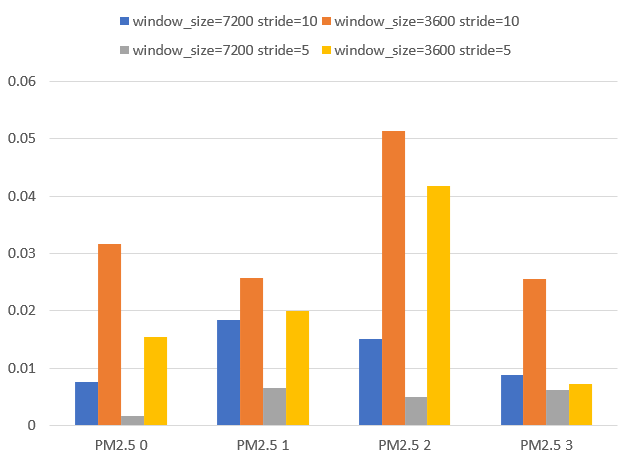
\includegraphics[width=0.8\linewidth]{fig/results/ablation/window_size3600_train_mse.png}
    \caption{Window size 7200 vs 3600.}
    \label{fig:window_size3600_train_mse}
\end{figure}

% \subsection{Compare with Other Methods}

\section{Conclusion}

The WaveNet model designed for audio data processing is generalizable and suitable for fitting problem. Our work successfully put it into usage for IAQI level fitting and prediction. It shows that our GreenEyes model based on WaveNet has strong data fitting capability for extreme long data sequences. When given a smaller stride, fed with more data, the model can learn better. It is also found that, when trained with more channels of sensor data, the model can perform well. This can be regard as sensor data augmentation. Our innovative method that human manually label the IAQI level is useful. It creates an appropriated target label function that the model can learn and solve the threshold fluctuation problem.

% The GreenEyes model fit well on the processed train data and also predict well on coordinated validation and test data. Both the MSE metric and MAE metric could converge into a small value.

% Furthermore, it comes from real scenario when users interact with this machine learning product and system.

% It is well tested that our GreenEyes AIoT system is dependable and have versatile applications. An app has been developed such that users could monitor the IAQI data in realtime when sensors are connected. GreenEyes deeplearning model can also be installed on the mobile and predict the IAQI level.

It is also promising that our GreenEyes AIoT deployment design can be put into practice. Actually we've developed an iOS app to retrieve the air quality data. Mobile framework such as Tensorflow Lite \cite{louis2019towards} has been developed. A mobile phone is hopefully to be installed with our GreenEyes model and monitor the IAQI data in realtime and predict the air trend.

Due to a lack of air quality data, we only did the data fitting task. We will perform the data predicting task in the future if enough data is gathered.

\section{Related Works}
\subsection{Statistical \& Machine Learning Approaches}

Except for ARIMA, ETS models mentioned in our last chapter, traditional methods such as Kalman filter \cite{gomez1994estimation} are also very simple and practical for time series and forecasting problems. Random forests \cite{rouet2017machine}, XGBoost, and SVM \cite{sapankevych2009time} etc are useful machine learning methods too. About method choosing, the most suitable method is highly interrelated with the data's properties and the application scenario. 

In common, the essential of both traditional approaches and ML-based approaches is mining data and extracting features. Different from other feature engineering tasks, sliding windows are widely used for processing the data. Metrics such as the minimum, the maximum, the mean, and the variance of the data in the window are common features.

\subsection{Deep Learning Approaches}

LSTM-based deep learning methods have been developed recently to extract temporal patterns. Lai et al. proposed LSTNet \cite{lai2018modeling} that encodes short-term local information into low dimensional vectors using 1D convolutional neural networks and decodes the vectors through an RNN. Shih et al. proposed TPA-LSTM \cite{shih2019temporal}  which processes the inputs by an RNN and employs a convolutional neural network to calculate the attention score across multiple steps.

The architecture of CNN is designed for 2D data like images. Meanwhile, recently a special variant of CNN called temporal convolutional networks (TCNs) \cite{lea2016temporal} has been proposed that makes CNN capable for time series processing. Yan et al. \cite{yan2020temporal} released their research work about using TCN for weather forecasting in 2020 and showed that TCN is better than the LSTM network in this application.

WaveNet related methods, including our GreenEyes model, tackle with a single sequence of time series data and show good fitting and forecasting performance concerning the prediction accuracy and data throughput capacity. Meanwhile, same with the same recent time as this thesis was being developed, new methods and approaches regarding time series forecasting have also been proposed. In recent years, graph neural networks (GNNs) have shown high capability in handling relational dependencies. Wu et al. \cite{wu2020connecting} proposed a general graph neural network framework designed specifically for multivariate time series data. Their method is useful for extracts relations among variables belonging to multi sequences.

As Transformer \cite{vaswani2017attention} becomes great popular these years, another model based on Transforms has also been brought out. Lim et al. \cite{lim2021temporal} from Google introduced the Temporal Fusion Transformer (TFT) as a novel attention-based architecture which combines high-performance multi-horizon forecasting with interpretable insights into temporal dynamics. They created gate-based networks, GRN and GLU, as new approaches for better feature selection modules.

\begin{acks}
The authors would like to thank many friends for constructive discussions and feedbacks. Special thanks to \href{https://www.math.hkust.edu.hk/people/faculty/profile/yuany/}{Prof. Yuan Yao} who voluntarily provides GPU machine.
\end{acks}

%%
%% The next two lines define the bibliography style to be used, and
%% the bibliography file.
\bibliographystyle{ACM-Reference-Format}
\bibliography{citations}

\end{document}
\endinput
%%
%% End of file `main-sigconf.tex'.
